\chapter{URG Equations for Generalised SIAM in Presence of Bath Correlation}

We will include a local particle-hole symmetric correlation of strength \(U_b\) on the origin of the lattice:
\begin{equation}\begin{aligned}
	\mathcal{H} = \sum_{k\sigma}\epsilon_k \tau_{k\sigma} + \epsilon_d \left( \hat n_{d \uparrow} - \hat n_{d \downarrow} \right) ^2 + \sum_{k\sigma} \left(V_{k} c^\dagger_{k\sigma} c_{d\sigma} + h.c.\right) +J \vec{S_d}\cdot\vec{s} + K \vec{C_d}\cdot\vec{C}- U_b\left(\hat n_{0 \uparrow} - \hat n_{0 \downarrow}\right)^2 
\end{aligned}\end{equation}

To treat this under RG, we first Fourier transform this term to \(k-\)space. In \(k-\)space, the diagonal contribution (to \(H_D\)) coming from this term is the single-particle self-energy \(-U_b\left(\hat n_{q \beta}\right)^2\) which can be made particle-hole symmetric in the form:
\begin{equation}\begin{aligned}
	-U_b\left(\tau_{q \beta}\right)^2
\end{aligned}\end{equation}
where \(q\) is the \(k-\)state being decoupled and \(\tau \equiv \hat n - 1/2\). In the initial state \(\ket{\Psi}_i\), we have \(\langle \hat n_{q\beta} \rangle = 1/2 \implies \tau_{q\beta} = 0\), so the contribution of \(U_b\) to that state is 0. For both hole excitations \(c_{q\beta}\ket{\Psi}_i\) as well as particle excitations \(c^\dagger_{q\beta}\ket{\Psi}_i\), the intermediate state energy lowers to \(-U_b/4\).

The off-diagonal part is
\begin{equation}\begin{aligned}
	-\frac{U_b}{2}\sum_{kk^\prime\sigma}c^\dagger_{k\sigma}c_{k^\prime\sigma} + U_b \sum_{k_1,k_2,k_1^\prime,k_2^\prime} c^\dagger_{k_1 \uparrow}c_{k_2 \uparrow} c^\dagger_{k^\prime_1 \downarrow}c_{k^\prime_2 \downarrow} 
\end{aligned}\end{equation}
We ignore the potential scattering arising from the first term.

\section{Renormalisation of \(U_b\)}
\(U_b\) can renormalise only via itself. The relevant renormalisation term in the particle sector is
\begin{equation}\begin{aligned}
	U_b^2 \sum_{q\beta}\sum_{k_1,k_2,k_3,k_1^\prime,k_2^\prime,k_3^\prime} c^\dagger_{q\beta}c_{k_1\beta}c^\dagger_{k_3\overline\beta}c_{k_1^\prime\overline\beta}\frac{1}{\omega - H_D}c^\dagger_{k_2^\prime\overline\beta}c_{k_3^\prime\overline\beta}c^\dagger_{k_2\beta}c_{q\beta}
\end{aligned}\end{equation}
In order to renormalise \(U_b\), we need to contract one more pair of momenta. There are two choices. The first is by setting \(k_3 = k_3^\prime = q\). The two internal states, then, are \(q\beta\) and \(q\overline\beta\). As discussed above, the intermediate state energy is \(-U_b/4\). We therefore have
\begin{equation}\begin{aligned}
	\frac{U_b^2 n_j}{\omega - D/2 + U_b/4}\sum_{\beta}\sum_{k_1,k_2,k_1^\prime,k_2^\prime} c_{k_1\beta}c_{k_1^\prime\overline\beta}c^\dagger_{k_2^\prime\overline\beta}c^\dagger_{k_2\beta} = \frac{U_b^2 n_j}{\omega - D/2 + U_b/4}\sum_{\beta}\sum_{k_1,k_2,k_1^\prime,k_2^\prime} c^\dagger_{k_2^\prime\overline\beta}c_{k_1^\prime\overline\beta}c^\dagger_{k_2\beta}c_{k_1\beta}
\end{aligned}\end{equation}
Another way to contract the momenta is by setting \(k_1^\prime = k_2^\prime = q\), which gives a renormalisation of
\begin{equation}\begin{aligned}
	\frac{U_b^2 n_j}{\omega - D/2 + U_b/4}\sum_{\beta}\sum_{k_1,k_2,k_3,k_3^\prime} c_{k_1\beta}c^\dagger_{k_3 \overline\beta}c_{k_3\prime\overline\beta}c^\dagger_{k_2\beta} = -\frac{U_b^2 n_j}{\omega - D/2}\sum_{\beta}\sum_{k_1,k_2,k_3,k_3^\prime} c^\dagger_{k_3 \overline\beta}c_{k_3\prime\overline\beta}c^\dagger_{k_2\beta}c_{k_1\beta}
\end{aligned}\end{equation}
The two contributions cancel each other. The same cancellation happens in the hole sector as well.

\section{Renormalisation of \(U\)}
\(U_b\) does not have any new renormalisation term on account of \(U_b\). \(U_b\) does however modify the existing RG equation for \(U\), by shifting the denominator. The existing RG equation is
\begin{equation}\begin{aligned}
	\Delta U &= -4V^2 n_j\left(\frac{1}{\omega - \frac{D}{2} + \epsilon_d + \frac{K}{4}} - \frac{1}{\omega - \frac{D}{2} - \epsilon_d + \frac{J}{4}}\right) - n_j\left(\frac{J^2}{\omega - \frac{D}{2} + \frac{J}{4}} - \frac{K^2}{\omega - \frac{D}{2} + \frac{K}{4}}\right)~.
\end{aligned}\end{equation}
On accounting for the contribution of \(U_b\) to the denominator, we get
\begin{equation}\begin{aligned}
	\Delta U &= -4V^2 n_j\left(\frac{1}{\omega - \frac{D}{2} + \frac{U_b}{4} + \epsilon_d + \frac{K}{4}} - \frac{1}{\omega - \frac{D}{2} + \frac{U_b}{4} - \epsilon_d + \frac{J}{4}}\right) - n_j\left(\frac{J^2}{\omega - \frac{D}{2} + \frac{U_b}{4} + \frac{J}{4}} - \frac{K^2}{\omega - \frac{D}{2} + \frac{U_b}{4} + \frac{K}{4}}\right)~.
\end{aligned}\end{equation}

\section{Renormalisation of \(V\)}
The single-particle  hybridisation \(V\) renormalises through terms of \(V U_b\) and \(U_b V\) kind. The first term gives
\begin{equation}\begin{aligned}
	&\sum_{q\beta}\sum_{k}U_b V c^\dagger_{q\beta}c_{k\beta} \hat n_{q\overline\beta} \frac{1}{\omega - H_D} c^\dagger_{d\beta}c_{q\beta} \\
	&= n_jU_b V\sum_{k\beta} c_{k\beta} \left[\frac{\hat n_{d\overline\beta}}{2}\left(\frac{1}{\omega_1 - E_1} + \frac{1}{\omega^\prime_1 - E_1}\right) + \frac{1-\hat n_{d\overline\beta}}{2}\left(\frac{1}{\omega_0 - E_0} + \frac{1}{\omega_0^\prime - E_0}\right)\right] c^\dagger_{d\beta}
\end{aligned}\end{equation}
\(E_1\) and \(E_0\) are the intermediate state energies for \(\hat n_{d\overline\beta}=1\) and 0 respectively. \(\omega_{1,0}\) are the quantum fluctuation scales for the corresponding initial states. \(\omega^\prime_{1,0}\) are the fluctuation scales for the corresponding final states.
The intermediate energies are \(E_1 = D/2 - U_b/4 - K/4,~ ~ ~ E_0 = D/2 - U_b/4 - U/2 - J/4\). The fluctuation scales are \(\omega_1 = \omega - U/2= \omega_0^\prime,~ ~ ~ \omega_1^\prime = \omega = \omega_0\). Substituting these gives
\begin{equation}\begin{aligned}
	-n_jU_b V\sum_{k\beta} c^\dagger_{d\beta} c_{k\beta} \left[\frac{\hat n_{d\overline\beta}}{2}\left(\frac{1}{\omega - \frac{D}{2} - \frac{U}{2} + \frac{U_b}{4} + \frac{K}{4}} + \frac{1}{\omega - \frac{D}{2} + \frac{U_b}{4} + \frac{K}{4}}\right) \right.\\
+\left. \frac{1-\hat n_{d\overline\beta}}{2}\left(\frac{1}{\omega - \frac{D}{2} + \frac{U_b}{4} + \frac{U}{2} + \frac{J}{4}} + \frac{1}{\omega - \frac{D}{2} + \frac{U_b}{4} + \frac{J}{4}}\right)\right]
\end{aligned}\end{equation}

The second term is of the form
\begin{equation}\begin{aligned}
	\sum_{q\beta}\sum_{k}U_b V c^\dagger_{q\beta}c_{d\beta} \frac{1}{\omega - H_D} \hat n_{q\overline\beta} c^\dagger_{k\beta}c_{q\beta}
\end{aligned}\end{equation}
and this is just the Hermitian conjugate of the previous term, so these two terms together lead to
\begin{equation}\begin{aligned}
	-n_jU_b V\sum_{k\beta} \left(c^\dagger_{d\beta} c_{k\beta} + \text{h.c.}\right) \left[\frac{\hat n_{d\overline\beta}}{2}\left(\frac{1}{\omega - \frac{D}{2} - \frac{U}{2} + \frac{U_b}{4} + \frac{K}{4}} + \frac{1}{\omega - \frac{D}{2} + \frac{U_b}{4} + \frac{K}{4}}\right) \right.\\
	+ \left.\frac{1-\hat n_{d\overline\beta}}{2}\left(\frac{1}{\omega - \frac{D}{2} + \frac{U_b}{4} + \frac{U}{2} + \frac{J}{4}} + \frac{1}{\omega - \frac{D}{2} + \frac{U_b}{4} + \frac{J}{4}}\right)\right]
\end{aligned}\end{equation}

In the hole sector, we have
\begin{equation}\begin{aligned}
	&\sum_{q\beta}\sum_{k}U_b V \hat n_{q\overline\beta} c^\dagger_{k\beta}c_{q\beta} \frac{1}{\omega - H_D} c^\dagger_{q\beta}c_{d\beta}\\
	&-\sum_{q\beta}\sum_{k}U_b V \left(1 - \hat n_{q\overline\beta}\right) c^\dagger_{k\beta}c_{q\beta} \frac{1}{\omega - H_D} c^\dagger_{q\beta}c_{d\beta}\\
	&= -n_jU_b V\sum_{k\beta} c^\dagger_{k\beta} \left[\frac{\hat n_{d\overline\beta}}{2}\left(\frac{1}{\omega_1 - E_1} + \frac{1}{\omega^\prime_1 - E_1}\right) + \frac{1-\hat n_{d\overline\beta}}{2}\left(\frac{1}{\omega_0 - E_0} + \frac{1}{\omega_0^\prime - E_0}\right)\right] c_{d\beta}
\end{aligned}\end{equation}
\(E_1 = D/2 - U_b/4 - U/2 - J/4,~ ~ ~ E_0 = D/2 - U_b/4 - K/4\). The fluctuation scales are \(\omega_1 = \omega = \omega_0^\prime,~ ~ ~ \omega_1^\prime = \omega - U/2 = \omega_0\). Substituting these gives
\begin{equation}\begin{aligned}
	-n_jU_b V\sum_{k\beta} c^\dagger_{d\beta} c_{k\beta} \left[\frac{1 - \hat n_{d\overline\beta}}{2}\left(\frac{1}{\omega - \frac{D}{2} - \frac{U}{2} + \frac{U_b}{4} + \frac{K}{4}} + \frac{1}{\omega - \frac{D}{2} + \frac{U_b}{4} + \frac{K}{4}}\right) \right.\\
+\left. \frac{\hat n_{d\overline\beta}}{2}\left(\frac{1}{\omega - \frac{D}{2} + \frac{U_b}{4} + \frac{U}{2} + \frac{J}{4}} + \frac{1}{\omega - \frac{D}{2} + \frac{U_b}{4} + \frac{J}{4}}\right)\right]
\end{aligned}\end{equation}
The other term, obtained by exchanging \(V\) and \(U_b\), gives the Hermitian conjugate, so the overall contribution from the hole sector is the same as the total contribution from the particle sector, but with \(\hat n_{d\overline\beta} \to 1 - \hat n_{d\overline\beta}\). Combining both the sectors, we get
\begin{equation}\begin{aligned}
	-n_jU_b V\sum_{k\beta} \left(c^\dagger_{d\beta} c_{k\beta} + \text{h.c.}\right) \frac{1}{2}\left[\left(\frac{1}{\omega - \frac{D}{2} - \frac{U}{2} + \frac{U_b}{4} + \frac{K}{4}} + \frac{1}{\omega - \frac{D}{2} + \frac{U_b}{4} + \frac{K}{4}}\right) \right.\\
+\left. \left(\frac{1}{\omega - \frac{D}{2} + \frac{U_b}{4} + \frac{U}{2} + \frac{J}{4}} + \frac{1}{\omega - \frac{D}{2} + \frac{U_b}{4} + \frac{J}{4}}\right)\right]
\end{aligned}\end{equation}

Combining with the already existing RG equations, the complete RG equation for \(V\) becomes
\begin{equation}\begin{aligned}
	\Delta V =& -\frac{3n_j V}{8}\left[\left(\frac{J}{\omega - \frac{D}{2} + \frac{U_b}{4} + \frac{J}{4}} + \frac{J}{\omega - \frac{D}{2} + \frac{U_b}{4} + \frac{U}{2} + \frac{J}{4}}\right) + K \left(\frac{K}{\omega - \frac{D}{2} + \frac{U_b}{4} + \frac{K}{4}} + \frac{K}{\omega - \frac{D}{2} + \frac{U_b}{4} - \frac{U}{2} + \frac{K}{4}}\right)\right]\\
		 &-\frac{n_jU_b}{2}\left[\left(\frac{V}{\omega - \frac{D}{2} - \frac{U}{2} + \frac{U_b}{4} + \frac{K}{4}} + \frac{V}{\omega - \frac{D}{2} + \frac{U_b}{4} + \frac{K}{4}}\right) + \left(\frac{V}{\omega - \frac{D}{2} + \frac{U_b}{4} + \frac{U}{2} + \frac{J}{4}} + \frac{V}{\omega - \frac{D}{2} + \frac{U_b}{4} + \frac{J}{4}}\right)\right]\\
		 &=-\frac{n_j V}{8}\left[\left(\frac{3J + 4U_b}{\omega - \frac{D}{2} + \frac{U_b}{4} + \frac{J}{4}} + \frac{3J + 4U_b}{\omega - \frac{D}{2} + \frac{U_b}{4} + \frac{U}{2} + \frac{J}{4}}\right) + \left(\frac{3K + 4U_b}{\omega - \frac{D}{2} + \frac{U_b}{4} + \frac{K}{4}} + \frac{3K + 4U_b}{\omega - \frac{D}{2} + \frac{U_b}{4} - \frac{U}{2} + \frac{K}{4}}\right)\right]
\end{aligned}\end{equation}

\section{Renormalisation of \(J\)}
We will track the entire renormalisation purely from that of \(J^+\), by virtue of the SU(2) symmetry. \(J^+\) renormalises through the \(J U_b\) terms. One of the terms is
\begin{equation}\begin{aligned}
	\frac{1}{2} J U_b \sum_{q} \sum_{k,k^\prime} S_d^+ c^\dagger_{q \downarrow} c_{k \uparrow} \frac{1}{\omega - H_D} \hat n_{q \uparrow} c^\dagger_{k^\prime \downarrow}c_{q \downarrow} = -\frac{1}{2}\frac{J U_b n_j}{\omega - \frac{D}{2} + \frac{U_b}{2} + \frac{J}{4}} \sum_{k,k^\prime} S_d^+ c^\dagger_{k^\prime \downarrow} c_{k \uparrow}
\end{aligned}\end{equation}
The factor of half in front is the same half factor that appears in front of the \(S_1^+ S_2^-, S_1^-S_2^+\) terms when we rewrite \(\vec{S}_1\cdot\vec{S}_2\) in terms of \(S^z, S^\pm\). Another term is obtained by switching \(J\) and \(U_b\):
\begin{equation}\begin{aligned}
	\frac{1}{2} J U_b \sum_{q} \sum_{k,k^\prime} \hat n_{q \downarrow} c^\dagger_{q \uparrow} c_{k \uparrow} \frac{1}{\omega - H_D}S_d^+ c^\dagger_{k^\prime \downarrow} c_{q \uparrow} = -\frac{1}{2}\frac{J U_b n_j}{\omega - \frac{D}{2} + \frac{U_b}{2} + \frac{J}{4}} \sum_{k,k^\prime} S_d^+ c^\dagger_{k^\prime \downarrow} c_{k \uparrow}
\end{aligned}\end{equation}

The corresponding terms in the hole sector are
\begin{equation}\begin{aligned}
	\frac{1}{2} J U_b \sum_{q} \sum_{k,k^\prime} S_d^+ c^\dagger_{k^\prime \downarrow} c_{q \uparrow} \frac{1}{\omega - H_D} \hat n_{q \downarrow} c^\dagger_{q \uparrow}c_{k \uparrow} = -\frac{1}{2}\frac{J U_b n_j}{\omega - \frac{D}{2} + \frac{U_b}{2} + \frac{J}{4}} \sum_{k,k^\prime} S_d^+ c^\dagger_{k^\prime \downarrow} c_{k \uparrow}
\end{aligned}\end{equation}
\begin{equation}\begin{aligned}
	\frac{1}{2} J U_b \sum_{q} \sum_{k,k^\prime} \hat n_{q \uparrow} c^\dagger_{k^\prime \downarrow} c_{q \downarrow} \frac{1}{\omega - H_D}S_d^+ c^\dagger_{q \downarrow} c_{k \uparrow} = -\frac{1}{2}\frac{J U_b n_j}{\omega - \frac{D}{2} + \frac{U_b}{2} + \frac{J}{4}} \sum_{k,k^\prime} S_d^+ c^\dagger_{k^\prime \downarrow} c_{k \uparrow}
\end{aligned}\end{equation}

Adding all these terms and combining with the existing RG equation, we get the updated RG equation for \(J\):
\begin{equation}\begin{aligned}
	\Delta J = -J n_j\frac{4 U_b + J}{\omega - \frac{D}{2} + \frac{U_b}{2} + \frac{J}{4}}
\end{aligned}\end{equation}

\section{Renormalisation of \(K\)}
We will follow the same strategy with \(K\) - we will calculate the renormalisation in \(K^+\). The first term is
\begin{equation}\begin{aligned}
	\frac{1}{2} K U_b \sum_{q} \sum_{k,k^\prime} \hat n_{q \downarrow} c^\dagger_{q \uparrow}c_{k^\prime \uparrow} \frac{1}{\omega - H_D} C_d^+ c_{k \downarrow} c_{q \uparrow} = -\frac{1}{2}\frac{K U_b n_j}{\omega - \frac{D}{2} + \frac{U_b}{2} + \frac{K}{4}} \sum_{k,k^\prime} C_d^+ c_{k \downarrow} c_{k^\prime \uparrow}
\end{aligned}\end{equation}
The second term in the same sector is obtained by flipping the spins of \(k\) and \(q\):
\begin{equation}\begin{aligned}
	\frac{1}{2} K U_b \sum_{q} \sum_{k,k^\prime} \hat n_{q \uparrow} c^\dagger_{q \downarrow}c_{k^\prime \downarrow} \frac{1}{\omega - H_D} C_d^+ c_{q \downarrow} c_{k \uparrow} = -\frac{1}{2}\frac{K U_b n_j}{\omega - \frac{D}{2} + \frac{U_b}{2} + \frac{K}{4}} \sum_{k,k^\prime} C_d^+ c_{k \downarrow} c_{k^\prime \uparrow}
\end{aligned}\end{equation}

The terms in the hole sector give identical contributions. The RG equation for \(K\) is
\begin{equation}\begin{aligned}
	\Delta K = -K n_j\frac{4 U_b + K}{\omega - \frac{D}{2} + \frac{U_b}{2} + \frac{K}{4}}
\end{aligned}\end{equation}

\section{Effect of tuning \(U_b = -U_0\)}

\begin{figure}[htpb]
	\centering
	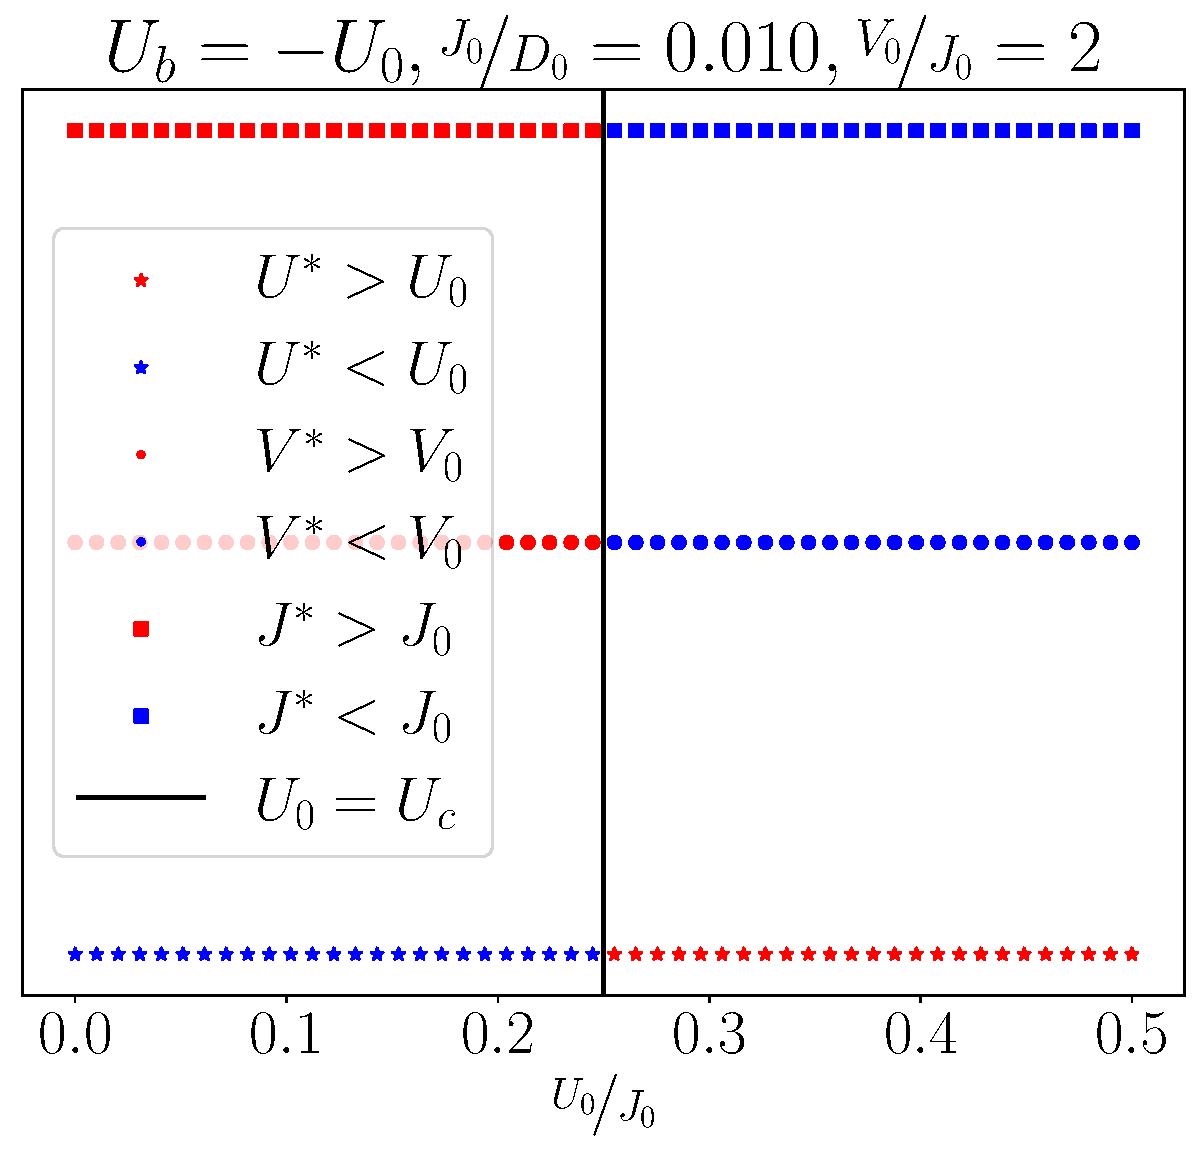
\includegraphics[width=0.6\textwidth]{../figures/MIT_with_Ub.pdf}
\end{figure}
The \(x-\)axis is the impurity correlation \(U\); we are keeping all other bare parameters fixed and increasing \(U\) while decreasing \(U_b\) using the constraint \(U_b = -U_0\). The black vertical line represents a certain value of the impurity correlation, \(U_c\). There are three horizontal sets of markers at variying heights; each set represents the fixed point values of a particular coupling. These couplings are \(U,V\) and \(J\) in order from bottom to top. If the marker is red, it means that the coupling is relevant there, whereas the marker being blue means the coupling is irrelevant. For \(U < U_c\), \(V\) and \(J\) are relevant while \(U\) is irrelevant, leading to a singlet ground state in the impurity problem and a metallic state in the bulk. For \(U > U_c\), \(J\) and \(V\) is irrelevant and \(U\) is relevant, so the ground state is a local moment on the impurity and an insulator in the bulk.
